\chapter{Introduction}

This chapter introduce the topic of the thesis. It defines the problem statement and also give a brief background about it.
\section{Background}
Denmark uses a social security number known as Central Personal Id (CPR Nr.) to provide digital identity to its citizens. Administrative data systems in Denmark currently rely on the CPR Nr. to link customer data with a real world identity. This means that almost all data managed by the institutions must be classified as personal identifiable information and therefore managed according to strict confidentiality requirements as well as integrity and availability requirements. This data is still vulnerable to insider threats, such as the recent leak of celebrity data from NETS to the magazine \textit{"Se \& Hør"}. However it is required by the authorities that the system should be able to link data with the real identity of the person, whenever there is some suspicion of criminal activity, e.g. fraud, insider trading, money laundering, etc.
\section{Motivation}
This thesis has been done in collaboration with 2 companies : \textit{Signicat} and \textit{Nykredit}.

Signicat is a provider of digital identity and digital signature solutions. They have the highest coverage of national electronic identities in Europe. They want to be able to offer services to financial institutions like Nykredit to help them in achieving the privacy goals regarding their customers.

Nykredit is a major financial institution in Denmark, providing different services, such as mortgages, retail banking, investment banking etc. They also are part of a big group of companies, which includes other financial institutions providing similar services. Currently there are 61 regional banks and partner institutions which have this partnership with Nykredit. These financial institutions basically provide Nykredit services as their own services to the customers.
Nykredit has mainly 2 types of customers:
\begin{enumerate}
\item Private Customers
\item Corporate Customers
\end{enumerate}
\subsection{Private Customers}
Private customers are the individual customers, who have personal bank account with  Nykredit and access their services themselves. Usually there is a single person accessing the services of the bank.
\subsection{Corporate Customers}
Corporate customers are either companies who are customers of Nykredit or other financial institutions which provide Nykredit services to their own private customers. In this case, there are many people who access Nykredit services on behalf of the corporate customer.
\section{Problem}
We consider the case of a person, who may be a private customer of Nykredit, and an employee of a company who is a corporate customer of the bank. For corporate customers, they have some employees who manage their bank account. In this case, the person may also be responsible for managing the accounts of his employer with Nykredit. This entity relationship is shown in the figure \ref{fig:Customers}.
\begin{figure}[h]
	\centering
	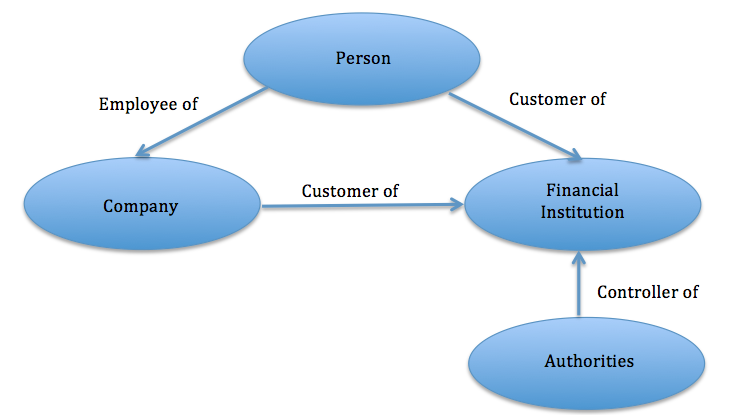
\includegraphics[width=\textwidth]{figures/Customers}
	\caption{Identities in the system}
	\label{fig:Customers}
\end{figure}

Nykredit wants to setup an identity management system so that there is no need for the individual to disclose his personal identity to Nykredit to access the account on behalf of the company.

Nykredit, however, also has to comply with relevant legislation (KYC, AML, “Hvidvaskningsloven”),  e.g. in case the authorities (Tax, Police, etc.) find some suspicious transactions. They need to provide the identity of the person responsible for these transactions.
This means that it is required that Nykredit, in case of a legal request, is able to identify the individual employee from the institution, who is accessing the account on the corporate customer’s behalf.
\\
\\So the main goal of the system is:
\begin{itemize}
	\item Nykredit should not learn identity of the individual person accessing the services on behalf of corporate customer.
	\item To comply with legislation Nykredit should be able to map the real identity of the individual person with the transaction, in case its required by the law.
\end{itemize}
In this thesis we will perform an initial analysis of a single business process from administrative data management, with respect to identifying the need to bind authenticated identities to actions at the different steps of the process; this analysis will be presented to stakeholders from the specific administrative domain. Based on the initial analysis of the selected business process, the project will develop a full identity model for the chosen business process with anonymisation and pseudonymisation of actors whenever possible. The feasibility of the proposed model will be evaluated through a prototype that implements the model using standard components from identity management infrastructures whenever possible.

Companies do not want to disclose the personal identity of their employees to Nykredit, but they still need the ability to access all services online. Managing all identities, while maintaining privacy, is not easy and provides different challenges. We have to design a system, which fulfill the entire privacy requirement and still enables Nykredit to provide its services to its customers and meet the regulatory requirements of the authorities without any problem.
 